\documentclass[journal]{IEEEtran}

\usepackage{amsmath,amsfonts,amssymb}
% \usepackage{algorithmic}
% \usepackage{array}
% \usepackage{textcomp}
% \usepackage{stfloats}
\usepackage{graphicx}
% \usepackage{xcolor}
% \usepackage{xspace}
% \usepackage{booktabs}
\usepackage{authblk}
\usepackage{url}
\usepackage{hyperref}
\usepackage{placeins}
\usepackage{caption}
\usepackage{subfigure}
\usepackage[maxcitenames=3,natbib=true,giveninits=true,backend=bibtex]{biblatex}
\addbibresource{bibliography.bib}
\usepackage{microtype}

\usepackage{booktabs} % for professional tables
\def\BibTeX{{\rm B\kern-.05em{\sc i\kern-.025em b}\kern-.08em
    T\kern-.1667em\lower.7ex\hbox{E}\kern-.125emX}}
\usepackage{balance}

\DeclareMathOperator*{\argmin}{arg\,min}
\DeclareMathOperator*{\argmax}{arg\,max}
\DeclareMathOperator*{\minimise}{\textrm{minimise}}
\DeclareMathOperator*{\maximise}{\textrm{maximise}}

\begin{document}
\title{A Training Rate and Survival Heuristic for Inference and Robustness Evaluation (TRASHFIRE)}
\author[1]{Charles Meyers}
\author[2]{Mohammad Reza Saleh Sedghpour}
\author[1]{Tommy L\"{o}fstedt}
\author[1]{Erik Elmroth}
\affil[1]{Department of Computing Science, Ume{\aa} University, {Ume\aa}, Sweden}
\affil[2]{Elastisys AB}


\maketitle
\begin{abstract}
Convolutional neural networks have shown to be widely applicable to a large number of fields when large amounts of labelled data are available. The recent trend has been to use models with increasingly larger sets of tunable parameters to increase model accuracy, reduce model loss, or create more adversarially robust models---goals that are often at odds with one another. In particular, recent theoretical work raises questions about the ability for even larger models to generalize to data outside of the controlled test and train sets. As such, we examine the role of the number of hidden layers in the ResNet model, demonstrated on the MNIST and CIFAR10 datasets. We test a variety of parameters including the size of the model, the floating point precision, and the noise level of both the training data and the model output. To encapsulate the model's predictive power and computational cost, we provide a modelling framework that uses induced failures to build an accelerated failure rate model. Using this novel approach, we are able to approximate the expected failure rate using a small number of specially crafted samples rather than increasingly larger benchmark datasets. We demonstrate the efficacy of this technique on both the MNIST and CIFAR10 datasets using 8-, 16-, 32-, 64-bit floating-point numbers, various data pre-processing techniques, and several attacks on 5 configurations of the ResNet model. Then, using empirical measurements, we examine the various trade-offs between cost, robustness, latency, and reliability to find that larger models do not significantly aid in adversarial robustness despite costing significantly more to train.
\end{abstract}
\section{Introduction}

Machine Learning (ML) has become a widely popular tool for solving complex problems across many disciplines, like medical imaging~\citep{ai_medical_imaging}, computer security~\citep{ai_security}, law enforcement~\citep{ai_prison}, aviation~\citep{ai_aviation}, and parcel scanning~\cite{ai_luggage}. Despite this, adversarial attacks aim to exploit vulnerabilities in machine learning models by introducing subtle modifications to data submitted to various stages of the ML pipeline, leading to misclassification or otherwise erroneous outputs~\citep{chakraborty_adversarial_2018}. Ensuring the robustness of ML models against adversaries has become a critical concern~\citep{adversarialpatch,carlini_towards_2017,croce_reliable_2020,hopskipjump,art2018,meyers}. However, understanding the relationship between computational cost and the performance against adversarial noise remains an ongoing challenge.  In this work, we investigated the robustness of various deep neural networks and data pre-processing techniques against adversarial attacks and explored the relationship between computational cost and  prediction accuracy in both benign and adversarial contexts.  By using samples crafted specifically to be challenging and applying accelerated failure rate models (see Sec.~\ref{afr_models}) we provide a method for estimating the expected failure time across the entire feasible adversarial space. Using this model, we demonstrate that larger models, while offering marginal gains over smaller models, do so at the expense of training times that far outpace the expected adversarial training time.

\subsection{Motivations}

It is routine to think in this adversarial context when considering safety- or security- critical applications~\cite{ai_medical_imaging,ai_security,ai_prison,ai_aviation,ai_luggage} where we assume the attacker is operating in their best-case scenario~\cite{leurent2020sha,kamal2017study,madry2017towards,pixelattack,deepfool,croce_reliable_2020}. A recent study~\cite{kamal2017study} distilled the process of password-cracking into an cloud-native service that can break common password schemes in a number of days. Another paper~\cite{leurent2020sha}, defines `broken' in the context of time to highlight the ease with which one can subvert a particular hashing algorithm. However, someone attacking a machine learning model might have a variety of competing goals that optimize the perturbation distance, number of queries, or other metrics~\cite{madry2017towards,hopskipjump,pixelattack,fgm,deepfool}. Much work has gone into mitigating the detrimental effects of these attacks, for example by adding noise in the training process~\cite{gauss_aug,gauss_out}, rejecting low-confidence results without penalty~\cite{high_conf}, or reducing the bit-depth of the data and model weights~\cite{feature_squeezing}. However, these analyses focus on ad-hoc posterior evaluations on benchmark datasets (namely CIFAR-10 and MNIST) to determine whether or not a given technique is more- or less-effective than another. That is, the relationship between marginal benefit and marginal cost is unclear. Furthermore, the community has relied on larger models~\cite{desislavov2021compute} and larger datasets~\cite{desislavov2021compute,bailly2022effects} to yield increasingly marginal gains~\cite{sun2017revisiting}. In order to reach safety-critical standards routine in other industries~\cite{iso26262,IEC61508,IEC62034}, we must move beyond the limited test/train split paradigm that would require many, many billions of samples for every change of a neural network~\cite{meyers}. So, first, we discuss failure rates and cost in the context of deep neural networks (see Section~\ref{cost}). Second, we demonstrate how to model the failure rate as a function of time  using accelerated methods (see Section~\ref{afr_models}). Third, we extend this time-dependent concept of `broken' algorithms from cryptography into machine learning (see Section~\ref{cost_normalization}). Using this, we can quickly and precisely investigate the effects of various attacks (see Section~\ref{attacks}), defences (see Section~\ref{defences}), and model architectures (see Section~\ref{models}).


\subsection{Contributions}

We summarize our contributions below:
\begin{itemize}
	\item We propose an accelerated failure time method for analyzing ML models under adversarial perturbations and provide substantial empirical evidence that this method is both effective and dataset-agnostic, allowing us to predict the expected failure rate more precisely and accurately than with either adversarial or benign accuracy alone.
	\item We use accelerated failure time models to measure model robustness across a wide variety of signal pre-processing techniques to explore the relationships between latency, accuracy, and model depth.
	\item We introduce a metric for evaluating whether or not a model is robust to adversarial attacks in a time- and compute-constrained context.
	\item We use this metric to show that, at best, increasing the number of hidden layers in a neural network increases training time while adding little-to-no benefit in the presence of an adversary.
\end{itemize}

\section{Background}


Much work has already gone into explaining the dangers of adversarial attacks on ML pipelines \citep{carlini_towards_2017,croce_reliable_2020,pixelattack,fgm,biggio_evasion_2013} though that work is limited to ad-hoc and posterior evaluations against limited sets of attack and defence parameters, leading to results that are, at best, overconfident~\citep{meyers,ma2020imbalanced}. Here, we are addressing \textbf{evasion}~\citep{carlini_towards_2017} attacks that attempt to induce a misclassification at run-time though our analysis extends to other types of attacks like database poisoning~\citep{biggio_poisoning_2013, saha2020hidden}, model inversion~\citep{choquette2021label,li2021membership}, or data stealing~\citep{orekondy2019knockoff}. This work formalizes methods for quantifying the adversarial failure rate of a model and comparing the efficacy of model changes in the context of fixed compute budget.

\subsection{Adversarial Attacks}

In the context of ML, an adversarial attack refers to deliberate and malicious attempts to manipulate the behavior of a model. These attacks are designed to change the model's behavior by introducing carefully crafted input data that can cause the model to make incorrect predictions or otherwise produce undesired outputs.
The goal of an attacker is often to exploit vulnerabilities in the model's decision-making process or to probe its weaknesses. These attacks can occur during various stages of the ML pipeline, including during training \citep{biggio_poisoning_2013}, inference\citep{biggio_evasion_2013}, or deployment \citep{santos2021universal}. For all sections below, we collect metrics on the benign (unperturbed) data and adversarial (perturbed) data. The abbreviations \textit{ben.} and \textit{adv.} are used throughout, respectively.


\subsubsection{Perturbation Distance}

\label{perturbation_distance}
The strength of an attack is generally thought of in terms of perturbation `distance'~\citep{croce_reliable_2020,chakraborty_adversarial_2018,pixelattack}. The perturbation distance, denoted by $\varepsilon$, quantifies the magnitude of the perturbation applied to a sample, $x$, when generating a new adversarial sample, $x'$. The definition is,
\[
    \varepsilon := \| x' - x \| \leq \varepsilon^*,
\]
where $\| \cdot \|$ denotes a norm or pseudo-norm (\textit{e.g.}, the Euclidean $\ell_2$ norm or the $\ell_0$ pseudo-norm). We denote by $\varepsilon^*$ the maximum allowed deviation or distortion from the original input while still being within the feasible sample space. For example, this might be one bit, one pixel, or one byte, depending on the test conditions. For more information on different optimization criteria, see Section~\ref{attacks}.


\subsubsection{Accuracy and Failure Rate}
The accuracy refers to the percentage or proportion of examples that cause the targeted ML model to misclassify or produce incorrect outputs and is a measure of the vulnerability or susceptibility of the model to noise-induced failures. A lower accuracy indicates a higher rate of misclassifications or incorrect predictions. The accuracy, $\lambda$, is defined as:
\begin{equation}
    \lambda := 1 -  \frac{\mathrm{False~Classifications}}{N},
    \label{eq:acc}
\end{equation}
where $N$ is the number of samples. The accuracy on a given test set, presumed to be drawn from the same distribution as the training set, is called the \textbf{benign accuracy}, $\lambda_{ben.}$. The \textbf{adversarial accuracy}, $\lambda_{adv.}$, is a measure of false classifications in the presence of noise intended to be adversarial. However, accuracy is known to vary with things like model complexity~\cite{vgg,resnet}, data resolution~\cite{feature_squeezing}, the number of samples~\cite{vapnik1994measuring}, the number of classes ~\cite{dohmatob_generalized_2019} or the amount of noise in the data~\cite{gauss_aug,gauss_out,dohmatob_generalized_2019}. Likewise, many of these factors can also influence an attack's run time. Instead, we can think in terms of \textbf{failure rate}:
\begin{equation}
    \mathrm{Failure~Rate} := \frac{\mathrm{False~Classifications}}{\Delta t} ,
    \label{eq:failure_rate}
\end{equation}
where $\Delta t$ is a time interval. This failure rate varies as a function of time, and we would like to model this behaviour with respect to various attributes and parameters of a model.
So, let $h$ be a function with model/attack parameters, $\theta$, such that $h_{\theta}$ describes the rate of failure at time $t$.
We can express the failure rate in terms of a \textbf{hazard function}, which can be expressed in terms of a point in time, $t$. It is defined as:
\begin{equation}
    h_{\theta}(t) := \lim_{ \Delta t \rightarrow 0} \frac{P(t \leq T < t + \Delta t \,|\, T \geq t)}{\Delta t},
    \label{eq:failure_rate_h}
\end{equation}
where $T$ is time until a false classification occurs, also referred to as \textbf{survival time}~\cite{kleinbaum1996survival}. To describe the computational efficacy of different model and attack configurations in general, we modelled the
probability of not observing a failure before a given time, $t$, giving the \textbf{cumulative survival function},
\begin{equation}
    S_{\theta}(t) := \exp \left\{- \int_0^{t} h_{\theta}(\tau) d\tau) \right\}.
    % := \exp( - H_{\theta}(t)), 
\label{eq:cdf}
\end{equation}
% as well as the \textbf{cumulative hazard function}, $H(t)$.
The probability density of observing a failure at time, $t$, is~\cite{kleinbaum1996survival},
\begin{equation*}
    f(t; \theta) := h_{\theta}(t)S_{\theta}(t).
    \label{eq:pdf}
\end{equation*}
\cm{In practice, $h_{\theta}(t), S_{\theta}(t)$ and/or $f(t; \theta)$ can be calculated if one of them is known ~\cite{kleinbaum1996survival}}.
% If we assume the probability of failure and time-to-failure is uniform across the samples\footnote{We don't use this assumption elsewhere---this is only mentioned to develop an intuition about the relationship between test set accuracy, the language of survival analysis, and the adversarial/benign distinction.} for a particular set of covariates, we can estimate the probability of failure on the unperturbed test set,
% \begin{equation}
%     f_{ben.}(t; \theta) \approx \frac{1 - \lambda_{ben.}}{t_{predict}} \cdot t,
%     \label{eq:ben_failure_rate}
% \end{equation}
% where $t_{predict}$ indicates the inference time per sample. As we can plainly see, at $t=t_{predict}$, this reduces to one minus the test-set \textbf{benign accuracy}. However, this is, at best, an optimistic lower bound to the the real-world failure rate~\cite{meyers,croce_reliable_2020}. To get a realistic picture of the worst-case scenario, we can look at $f$ in the presence of adversarial noise,
% \begin{equation}
%     f_{adv.}(t; \theta) \approx \frac{ 1 - \lambda_{adv.}}{t_{attack}} \cdot t,
%     \label{eq:adv_failure_rate}
% \end{equation}
% where $t_{attack}$ refers to the attack generation time per sample. Hence, at $t=t_{attack}$ this reduces to one minus the \textbf{adversarial accuracy}.


\subsection{Cost}

\label{cost}
For our purposes, we assumed the cost, $C_{train}$, is proportional to the total training, $T_{train}$, the number of samples, $N$,  and the training time per sample, $t_{\mathrm{train}}$, such that the cost of training on hardware with a fixed time-cost, $C_h$, is
\[
    C_{train} := C_{h} \cdot T_{\mathrm{train}} = C_h \cdot t_{train} \cdot N,
\]
where $C_h$ is the cost per time unit of a particular piece of hardware. This assumption means that cost will scale linearly with per-sample training time or sample size. Analogously, we can discuss this in adversarial terms where $N$ is the number of samples. If we assume the same hardware cost as the model-builder then,
$$
    C_{attack} := C_{h} \cdot T_{\mathrm{attack}} = C_h \cdot t_{attack} \cdot N.
$$

If we assume that the training time and attack time are uniform across the samples and restricted to the same hardware, then we can say that
\begin{equation}
C_{train} \propto t_{train} \text{~~~and~~~} C_{attack} \propto t_{attack}.
\label{eq:naive_cost}
\end{equation}

Furthermore, a fast attack will be lower-bounded by $t_{predict}$, which is generally much smaller than the training time, $t_{train}$. Of course the long-term costs of deploying a model will be related to the inference cost, but a model is clearly broken if the cost of improving a model ($\propto t_{train}$) is much, much larger than the cost of finding a counterexample ($\propto t_{attack}$) within some imperceptible noise distance of untainted samples. However, this merely encapsulates the cost of a particular model architecture or signal pre-processing choice and doesn't consider the likelihood of noise induced failure. Our cost normalized metric is introduced below in Eq.~\ref{eq:cost} in Section~\ref{cost_normalization}. Before we can compare this cost to the failure rate, we must estimate the attack time per sample, or expected survival time, $\mathbb{E}[T]$. For that, we use an accelerated failure rate model.


\section{Survival Analysis for ML} 
\label{afr_models}
Failure rate analysis has been widely explored in other fields~\cite{aft_models} from medicine to industrial quality control~\cite{ai_medical_imaging,ai_industry,ai_aviation,ai_luggage,ai_security,ai_prison}, but there's very little published research in the context of ML. However, as noted by many researchers~\cite{madry2017towards, carlini_towards_2017, croce_reliable_2020, meyers}, these models are fragile to attackers that intend to subvert the model, steal the database, or evade detection.  In this work, leverage evasion attacks to examine their time-to-failure   that model the survival time or time to failure, $S_{\theta}(t)$ for a model with covariates, $\theta$. For all survival models we can use the survival function to compute the expected survival time,
\[
	\mathbb{E}_{S_\theta}[T] = \int_0^{\infty}S_\theta(t) \,dt.
\]
For the purposes of inferential statistics, we can broadly separate these models into two categories: proportional hazard models and accelerated failure time models, each of which has a subsection below. Furthermore, by parameterizing our performance with time, we are able to do the cost-value analysis outlined in Sec.~\ref{cost_normalization}.

\subsection{Proportional Hazard Models}
Proportional hazard models try to fit a parameter $\phi$ to a matrix of covariates, $\theta$, to predict the survival time on unseen configurations of covariates or used for inferential statistics, such that
$$
S_\theta(t) = S_0(t) \cdot \phi(\theta, x), 
$$
where $\phi$ is a \textit{proportional hazard} that depends on the covariates, typically $\phi(\theta, x) = \exp{(\theta_1 x_1 + \theta_2 x_2 + \cdots + \theta_p x_p)}$ and $S_0$ is the baseline survivor function. For example, the covariates might be things like perturbation distance, model depth, or number of training epochs.


\subsubsection{Cox}
One example of proportional hazard models is the Cox variety, which can be defined in terms of the hazard function:
$$
h(t) = h_0(t) \cdot \exp(\phi_1 \theta_1 + \phi_2 \theta_2... \phi_p \theta_p)
$$
where $\phi_p$ is the $p$-th proportional hazard coefficient and $\theta_p$ is the value of the $p$-th covariate. One downside of Cox compared to the other models is that it is semi-parametric since $h_0(t)$ is not defined by a parametric model. Furthermore, this means that $\phi_1, \phi_2... \phi_p$ are only defined for a particular dataset and only describe the proportional effect of the covariates rather than the more general acceleration factor discussed in the next section.


\subsection{Accelerated Failure Time Models}
\cm{Note: This subsection has been re-written.}

Accelerated Failure Rate (AFR) models have been widely used to investigate the causes and likelihood of failures across fields where safety is a primary concern (\textit{e.g.}, in medicine, aviation, or automobiles)~\cite{liu2013development,lawless1995methods}. For manufacturing, this is n done by accelerating normal wear and tear on a particular component (e.g. a motor or aircraft sensor)~\cite{liu2013development}. For the study of diseases in humans, these models are often build on demographic data and used to examine the effect of various things on the expected lifetime of an individual. For machine learning, we can leverage the worst-case perturbations of an adversary to model the effect of various model parameters for both predictive and inferential statistics. That is, they can successfully estimate the expected survival time of a component using statistical methods and routine results from model training. These accelerated models are of the form:
$$
	S_\theta(t) = S_0(\phi(\theta, x) \cdot t).
$$
where $\phi$ is an \textit{acceleration factor} that depends on the covariates, typically $\phi(\theta, x) = \exp{(\theta_1 x_1 + \theta_2 x_2 + \cdots + \theta_p x_p)}$ and $S_0$ is the baseline survivor function. For example, the covariates might be things like perturbation distance, model depth, or number of training epochs.

\subsubsection{Generalised Gamma}
The generalised gamma model uses three parameters $\sigma, \lambda,\gamma$. Let

$$
u (x,y)= \Gamma \left ( \frac{1}{(\lambda(x, \alpha))^2}; \frac{\exp \left( \lambda(x, \alpha) \left( \frac{log(t) - \mu(\gamma, x)}{\sigma(\beta, y)} \right ) \right) }{(\lambda(x, \alpha))^2} \right )
$$
where $\Gamma(k, x)$ is the incomplete Gamma function$ \lambda(x, \alpha) = \alpha x^T, \sigma(\beta, y) = \exp(\beta y ),   \mu(\gamma, x) = \gamma x^T$, and $\theta = (\lambda, \sigma, \mu) $~\cite{aft_models}. Then we can express the survival function as a piece-wise function:
$$
S_{\theta}(t; x, y) =  1 - u~\text{when}~\lambda > 0 
$$
and
$$
S_{\theta}(t; x, y) =  u~\text{when}~\lambda \leq 0 .
$$ 
The exponential, Weibull, and log-normal models outlined below are all special cases of this model ~\cite{kleinbaum1996survival}.

\subsubsection{Exponential Model}
The exponential survival model can be defined in terms of the cumulative survival function:
$$
S_{\theta}(t; x, y) = \exp \left( -\frac{t}{\lambda_0 \cdot \exp(\beta x + \gamma y)} \right)
$$
where $\beta, \gamma$ are the coefficients associated with the vector of covariates, $x$, the vector of failure events, $y$ and $\theta = (\alpha, \beta, \gamma)$

\subsubsection{Weibull AFR}
The first AFR model we tested was using the Weibull distribution, which has the form
\[
	S_\theta(t; x, y) = \exp{\left( - \left( \frac{t}{\lambda(\beta, x)} \right)^{\rho(\alpha, y)} \right)},
\]
where $\theta=(\alpha, \beta)$, $\lambda(\beta, x)=\exp(\beta_0 + \beta_1 x_1 + \cdots + \beta_n x_p)$ is a scale parameter, and $\rho(\alpha, y)=\exp(\alpha_0 + \alpha_1 y_1 + \cdots + \alpha_p y_p)$ is a shape parameter that determines the direction of acceleration over time.

\subsubsection{Log-Normal AFR}

The Log-Normal AFR model introduces the parameters $\mu(\alpha, x) = \alpha_0 + \alpha_1 x_1 + \cdots + \alpha_n x_p $ and $\sigma(\beta, y) = \exp(\beta_0 + \beta_1 y_1 + \cdots + \beta_n y_p)$ with the survival function given by,
\[
	S_\theta(t; x, y) = 1 - \log \left( 1 - \Phi \left (  \frac{\log(t) - \mu(\alpha, x) }{ \sigma(\beta, y) } \right) \right).
\]



\subsubsection{Log-Logistic AFR}

Another form of the AFR model, the Log-Logistic AFR, introduces the scale and shape parameters $a(\alpha, x) = \exp(\alpha_0 + \alpha_1 x_1 + \cdots + \alpha_n x_p )$ and $b(\beta, y) = \exp(\beta_0 + \beta_1 y_1 + \cdots + \beta_n y_p)$, respectively, with survival function,
\[
	S_\theta(t; x, y) = 1 - \log \left( 1 + \left (  \frac{t - a(\alpha, x) }{ b(\beta, y) }\right)\right),
\]
where $\theta = (\alpha, \beta)$.



\subsection{\cm{Survival Model Validation}}
\label{metrics}

To compare the efficacy of different parametric aft models, we use the Akaike information criterion (AIC) and the Bayesian information model ~\cite{stoica2004model,taddy2019business}, \cm{where the preferred model will be the one with the smallest value. In addition to these metrics, we also include the 
concordance score, which is equivalent to the area under (AUC) the receiver operating characteristic curve (ROC)~\cite{pantoja2021concordance}.} In particular we note that a concordance index $> .5$ indicates that the failure rate is a function of time, undermining the efficacy of the time-independent train/test split methodology that is standard in the literature \cite{concordance}.\cm{Following recent research~\cite{ici}, we also include graphical calibration curves (see Fig.~\ref{fig:afr_models}), which depict the relationship between our fitted model (y-axis) and a model fit to the data using cubic splines (x-axis) as in this paper~\cite{ici}. In addition, we
the mean difference between the predicted and observed failure probabilities (e.g. integrated calibration index or ICI) and the median value of these differences (e.g. the error at the 50th percentile or the E50). TODO: mention log likelihood ratio.}





\section{Failure Rates and Cost Normalisation}


\label{cost_normalization}


So, finally, we can introduce the idea of a failure rate normalised cost, or training time to attack time ratio. If we assume that the cost scales linearly with $t_{train}$ (Eq.~\ref{eq:naive_cost}), then we can normalise it by the expected survival time to get a rough estimate of the costs for the model builder ($C_{train} \propto T_{train}$) or the attacker ($C_{adv.} \propto \mathbb{E}_{S_\theta}[T] \approx t_{attack}$). Recalling the definition of $\varepsilon$ from Eq.~\ref{eq:perturbation_distance}, we can separately consider the cases $\varepsilon=0$ and $\varepsilon > 0$. Then, we can express this cost of failure in both benign and adversarial terms as,
\begin{equation}
	\bar{C}_{ben.} = \frac{T_{train}}{\mathbb{E}_{S_\theta}[T \,|\, \varepsilon = 0] }
	\text{~~and~~}
	\bar{C}_{adv.}=\frac{T_{train}}{\mathbb{E}_{S_\theta}[T \,|\, 0 < \varepsilon \leq \varepsilon^*]}.
	\label{eq:cost}
\end{equation}
If $\bar{C} \gg 1$ (in either case) then it's clear that our approach is invalid (\textit{i.e.}, that our model is \textit{broken}), because it is cheaper to attack the model than it is to train it. Also, if you treat $\varepsilon$ as a covariate in ${S_\theta}(t)$, then these costs can be computed from the same model.
This approach has two advantages over the traditional train-test split method. Firstly, we can quantify the effects of covariates like model depth or noise distance to compare the effect of model changes. Secondly, the train-test split methodology relies on an ever-larger number of samples to increase precision, whereas the accelerated failure method is able to precisely and accurately compare models using only a small number of samples~\cite{schmoor2000sample,lachin1981introduction} relative to the many billions required of the train/test split methodology and safety-critical standards~\cite{iso26262,IEC61508,IEC62034,meyers}. 
In short, by generating worst-case examples (\textit{e.g.}, adversarial ones), we can test \textit{and compare} arbitrarily complex models \textit{before} they leave the lab, drive a car, predict the presence of cancer, or pilot a drone. 
\section{Methodology}
\label{methods}
Below we outline the experiments performed and the hyper-parameter configurations of the models, attacks, and defences across the various model architectures, model defences, and attacks. All experiments were conducted on Ubuntu 18.04 in a virtual machine running in a shared-host environment with one NVIDIA V100 GPU using Python 3.8.8. All configurations were tested in a grid search using \texttt{hydra}~\cite{hydra} to manage the parameters, \texttt{dvc}~\cite{dvc} to ensure reproducibility, and \texttt{optuna}~\cite{optuna} to manage the scheduling. For each attack and model configuration, we collected the metrics outlined in Equations~\ref{eq:acc}--\ref{eq:cost} as well as the inference time, training time, and attack generation time. We conducted a grid search of datasets, models, defences, and attacks across ten permutations of the data. For visualization, we approximated $f_{\mathrm{ben.}}$ and $f_{\mathrm{adv.}}$ for each attack and defence combination using Equation~\ref{eq:failure_rate} and approximated $\bar{C}$ in the adversarial and benign scenarios as per Equation~\ref{eq:cost}.


\subsection{Dataset}
\label{dataset}

Experiments were performed on both the CIFAR100, CIFAR10~\cite{cifar}, and MNIST~\cite{mnist} datasets. We measured the adversarial/benign accuracies, the attack generation time, and the prediction time. To calculate the adversarial failure rate and the cost we used Equations.~\ref{eq:failure_rate}~\&~\ref{eq:cost}. For accuracy, see: Equation~\ref{eq:acc}. We trained on 80\% of the samples for all datasets. Of the remaining 20\%, one-hundred class-balanced samples were selected from this test set to evaluate each attack. In addition, the data were shuffled to provide us with 10 samples for each configuration. Then, the data were centered and scaled by the using the parameters defined by the training set to avoid data leakage and to give a more obvious interpretation to different values of $\varepsilon$.


\subsection{Tested Models}
\label{models}

The Residual Neural Network (ResNet)~\cite{resnet} is a popular classification model\footnote{More than 180 thousand citations: \href{https://scholar.google.com/scholar?cites=9281510746729853742}{ResNet citations on Google Scholar.}} because of its ability to train neural networks with many layers efficiently through \textit{residual connections}.
\textit{Deep} networks, \textit{e.g.}, VGG~\cite{vgg}, ResNet~\cite{resnet}, rely on the depth of the network, which, despite leading to more accurate or robust results~\cite{rolnick2017power, carlini_towards_2017}, tends to lead to the `vanishing gradient problem'~\cite{hochreiter1998vanishing}, making learning difficult and slow. However, the residual connections allow models to have hundreds of layers rather than tens of layers~\cite{resnet,vgg}. Despite the prevalence of the reference architecture, several modifications have been proposed that trade off, for instance, robustness and computational cost by varying the number of convolutional layers in the model. We tested the \textbf{Resnet-18}, \textbf{-34}, \textbf{-51}, \textbf{-101}, and \textbf{-152} reference architectures, that get their names from their respective number of layers. We used the the \texttt{pytorch} framework and the Stochastic Gradient Descent minimiser with a momentum parameter of 0.9 and learning rates $\in \{10, 1, 0.1, 0.01, 0.001, 0.0001, .00001, 0.000001\}$ for epochs $\in \{ 10, 20, 30, 50, 100\}$. The learning rate that maximised the benign accuracy for a given layer/defence configuration was used in further analyses (\textit{i.e.}, the learning rate was tuned). In a separate experiment, we also evaluated the different Resnet models across epochs $\in \{10, 20, 30, 50, 100\}$.

\subsection{Tested Defences}
\label{defences}

In order to simulate various conditions affecting the model's efficacy, we have also tested several defences that modify the model's inputs or predictions in an attempt to reduce its susceptibility to adversarial perturbations. Just like with the attacks, we used the Adversarial Robustness Toolbox~\cite{art2018} for their convenient implementations. These defences are listed below.

\textbf{Gauss-in} ($\ell_2$): The 'Gaussian Augmentation' defence adds Gaussian noise to some proportion of the training samples. In our case, we set this proportion to 50\%, allowing us to simulate the effect of noise on the resulting model~\cite{gauss_aug}. We tested noise levels in $\{.001, .01, .1, .3, .5, 1\}$.

\textbf{Conf} ($\ell_{\infty}$): The 'High Confidence Thresholding' defence only returns a classification when the specified confidence threshold is reached, resulting in a failed query if a classification is less certain. This allows us to simulate the effects of rejecting 'adversarial' or otherwise 'confusing' queries~\cite{high_conf} that fall outside the given confidence range by ignoring ambiguous results without penalty. We tested confidence levels in $\{.1, .5, .9, .99, .999\}$.

\textbf{Gauss-out} ($\ell_2$): The 'Gaussian Noise' defence, rather than adding noise to the input data, adds noise to the during inference~\cite{gauss_out}, allowing us to reduce precision to grey- and black- box attacks without going through costly training iterations. We tested levels in $\{.001, .01, .1, .3, .5, 1\}$. 

\textbf{FSQ}: The 'Feature Squeezing' defence changes the bit-depth of the input data to minimise the noise induced by floating-point operations. We include it here to simulate the effects of various GPU or CPU architectures, which may also vary in bit-depth~\cite{feature_squeezing}. We tested bit-depths in $\{2, 4, 8, 16, 32, 64\}$.



\subsection{Tested Attacks}
\label{attacks}

In order to simulate various attacks that vary in information and run-time requirements across a variety of distance metrics, we have evaluated several attacks using the Adversarial Robustness Toolbox~\cite{art2018}. Other researchers~\cite{carlini_towards_2017} have noted the importance of testing against multiple types of attacks. For our purposes, \textbf{attack strength} refers to the degree to which an input is modified by an attacker, as described in Sec.~\ref{perturbation_distance}. Below, we briefly describe the attacks that we tested against. One or more norms or pseudo-norms were used to optimise each attack, denoted in the parentheses next to the attack name. 

\textbf{FGM} ($\ell_1, \ell_2, \ell_{\infty}$): The 'Fast Gradient Method' quickly generates a noisy sample with no feasibility conditions beyond a specified step size and number of iterations~\cite{fgm} by using the model gradient and taking a step of length $\varepsilon$ in the direction that maximises the loss with $\varepsilon \in \{.001,.01,.03,.1,.2,.3,.5,.8,1\}$.

\textbf{PGD}  ($\ell_1, \ell_2, \ell_{\infty}$): The 'Projected Gradient Method' extends the FGM attack to include a projection on the $\varepsilon$-sphere, ensuring that generated samples do not fall outside of the feasible space~\cite{madry2017towards}. This algorithm is iterative, and we restricted it to ten such iterations. In short, this imposes feasibility conditions on the FGM attack with $\varepsilon \in \{.001,.01,.03,.1,.2,.3,.5,.8,1\}$.

\textbf{Deep} ($\ell_2$): the Deepfool Attack~\cite{deepfool} finds the minimal separating hyperplane between two classes and then adds a specified amount of perturbation to ensure it crosses the boundary by using an approximation of the model gradient including the top $n$ outputs where $n \in \{1,3,5,10\}$, speeding up computation by ignoring unlikely classes~\cite{deepfool}. This algorithm is iterative and we restricted it to ten such iterations.

 \textbf{Thresh} ($\ell_{\infty})$: the `Threshold' attack also uses the same multi-objective search algorithm as Pixel to optimise the attack, but tries to maximise false confidence while minimizing the $\ell_2$ perturbation distance. This algorithm is iterative and we restricted it to ten such iterations.
 
\textbf{HSJ} ($\ell_2$, \textit{queries}): the `HopSkipJump' attack, in contrast to the attacks above, does not need access to model gradients nor soft class labels, instead relying on an offline approximation of the gradient using the model's decision boundaries. In this case, the strength is denoted by the number of queries necessary to find an adversarial counterexample~\cite{hopskipjump}. This algorithm is iterative and we restricted it to ten such iterations.

\subsection{Identification of ResNet Model-, Defence- and Attack-Specific Covariates}
For each attack type, we identified the attack-specific distance metric (or pseudo-metric) outlined in Sec.~\ref{attacks}. To compare the effect of this measure against other attacks, the valued were min-max scaled so that all values fell on the interval $[0,1]$. For defences, we did the same scaling. However, while a larger number always means more (marginal) noise in the case of attacks, a larger value for the FSQ defence indicates a larger bit-depth and more floating point error. For Gauss-in and Gauss-out, a larger number does indicate more noise, but a larger number for Conf indicates a larger rejection threshold for less-than-certain classifications, resulting in less low-confidence noise. Therefore, we introduced a dummy variable for each attack and defence, allowing us to estimate their effect relative to the baseline hazard. For the models we tracked the number of epochs and the number of layers as well as the training and inference times.  


\subsection{AFR Models}
We tested the Weibull, Log-Normal, and Log-Logistic AFR models using the \texttt{lifelines}~\cite{lifelines} package in Python, relying on the metrics outlined in Section~\ref{metrics} for comparison since they are widely used in the AFR literature \cite{aft_models}.

\section{Results and Discussion}
\cm{Note: This section has been substantially rewritten.}
\label{results}
\begin{figure}[!h]
\begin{subfigure}
    \centering
    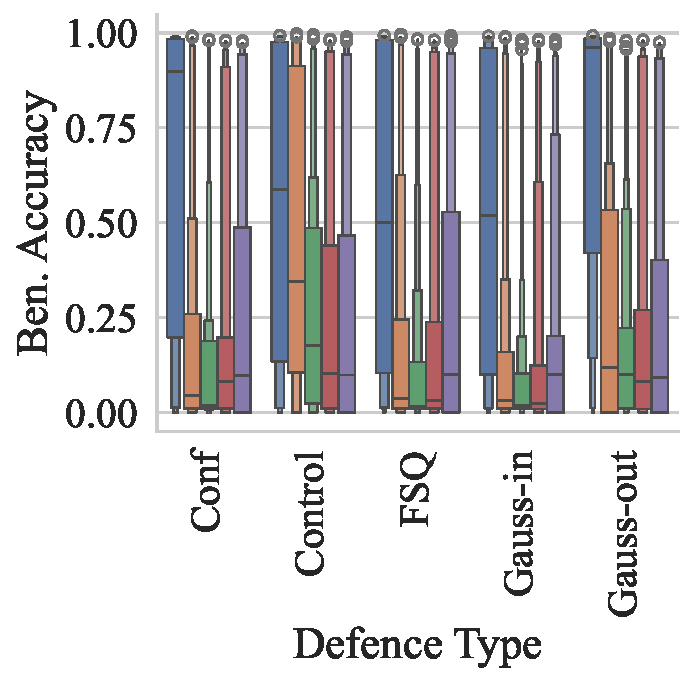
\includegraphics[trim={0 5pt 0 10pt},clip,width=.45\textwidth]{plots/ben_accuracy_vs_defence_type.pdf}
\end{subfigure}
\begin{subfigure}
    \centering
    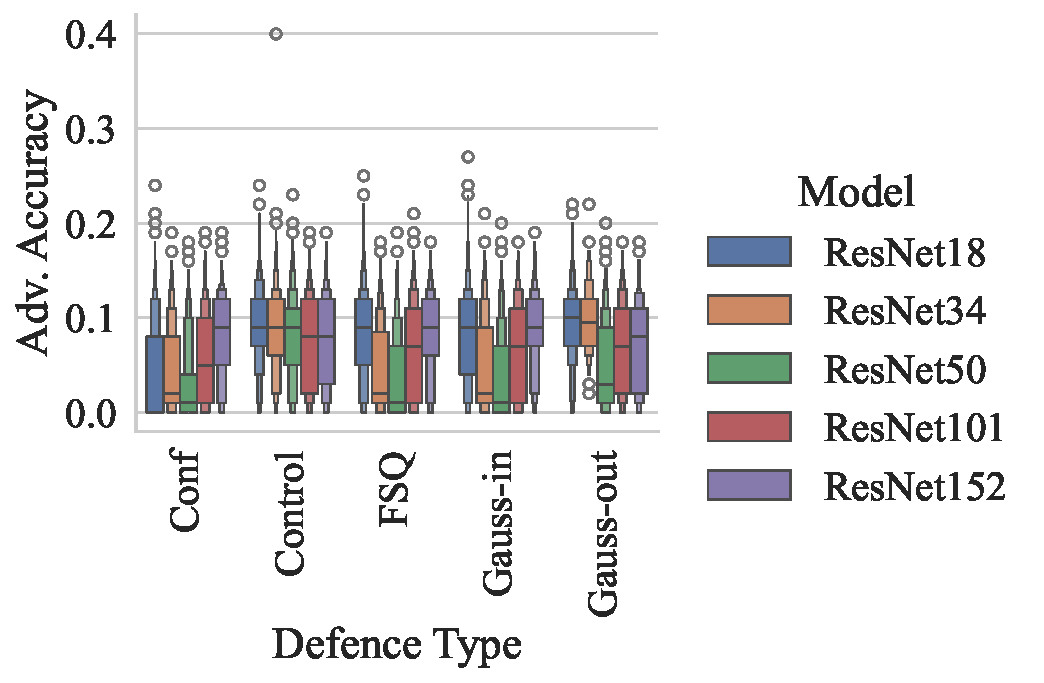
\includegraphics[trim={0 5pt 0 10pt},clip,width=.45\textwidth]{plots/adv_accuracy_vs_defence_type.pdf}
\end{subfigure}
\begin{subfigure}
    \centering
    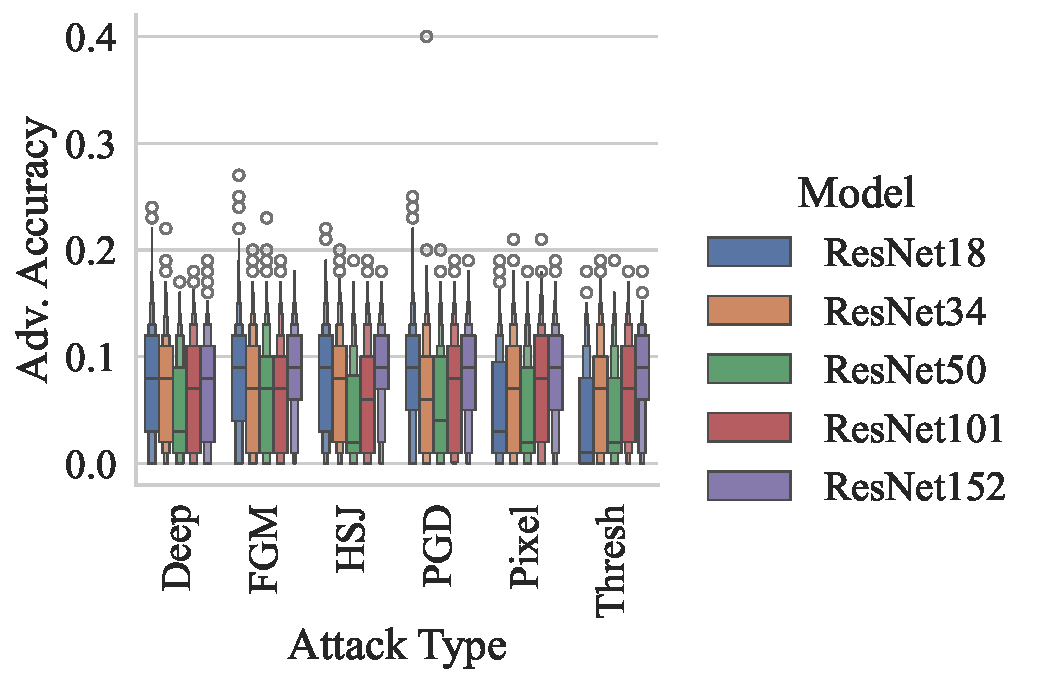
\includegraphics[trim={0 5pt 0 10pt},clip,width=.45\textwidth]{plots/adv_accuracy_vs_attack_type.pdf}
\end{subfigure}
\caption{The adversarial accuracy across various attacks pictured on the x-axis and outlined in Section~\ref{attacks}. The error bar reflects the 95\% confidence interval for the adversarial accuracy across all examined samples. The violin plots reflect the 95\% confidence intervals for each tuned hyperparameter combination. Outliers are indicated with a circle.}
\label{fig:accuracies}
\end{figure}

\begin{figure}[!h]
    \centering
    \begin{subfigure}
        \centering
        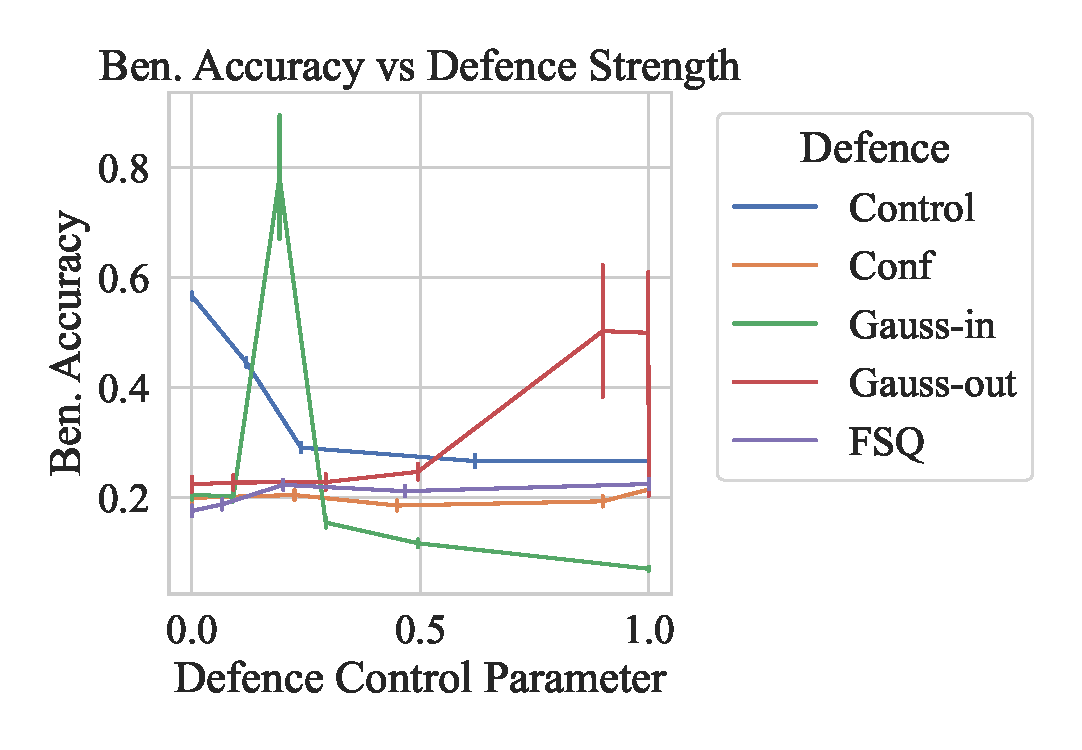
\includegraphics[trim={0 10pt 0 10pt},clip,width=.45\textwidth]{plots/def_param_vs_accuracy.pdf}
    \end{subfigure}
    \begin{subfigure}
        \centering
        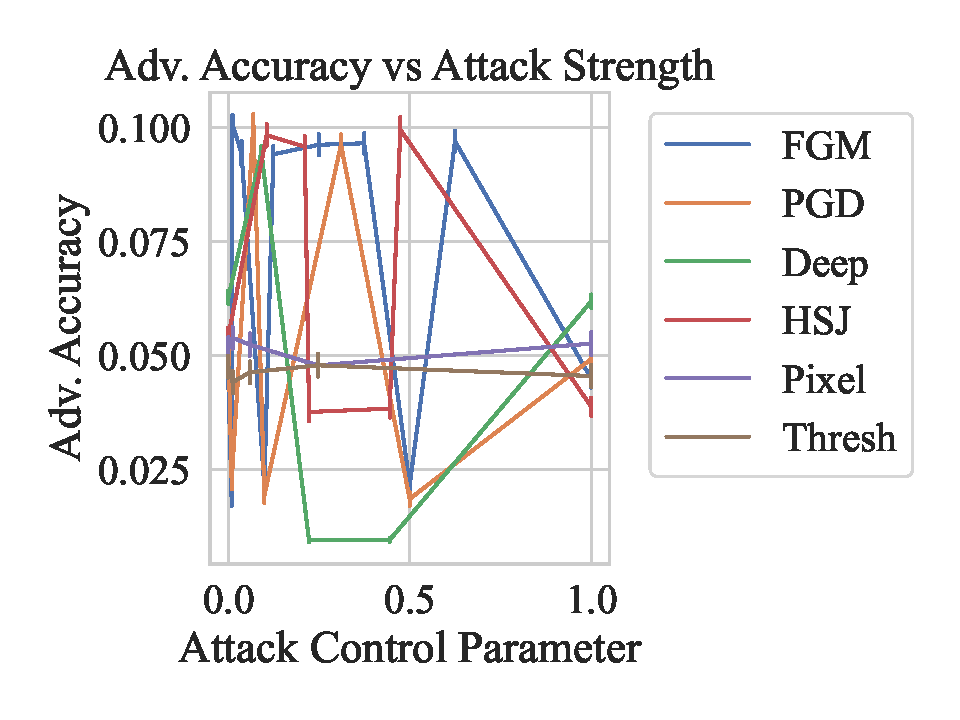
\includegraphics[trim={0 10pt 0 10pt},clip,width=.45\textwidth]{plots/atk_param_vs_accuracy.pdf}
    \end{subfigure}
    \caption{This depicts the benign (unperturbed) and adversarial (perturbed) failure rates across all defences attacks, and models. The left shows how the benign accuracy varies with the defence strength where the control parameter describes the number of layers. The right shows the adversarial accuracy as a function of attack strength. The bars indicate the first standard deviation of measures across all model configurations.}
    \label{fig:strength}
\end{figure}

% \begin{figure}[!h]
%     \centering
%     \begin{subfigure}
%         \centering
%         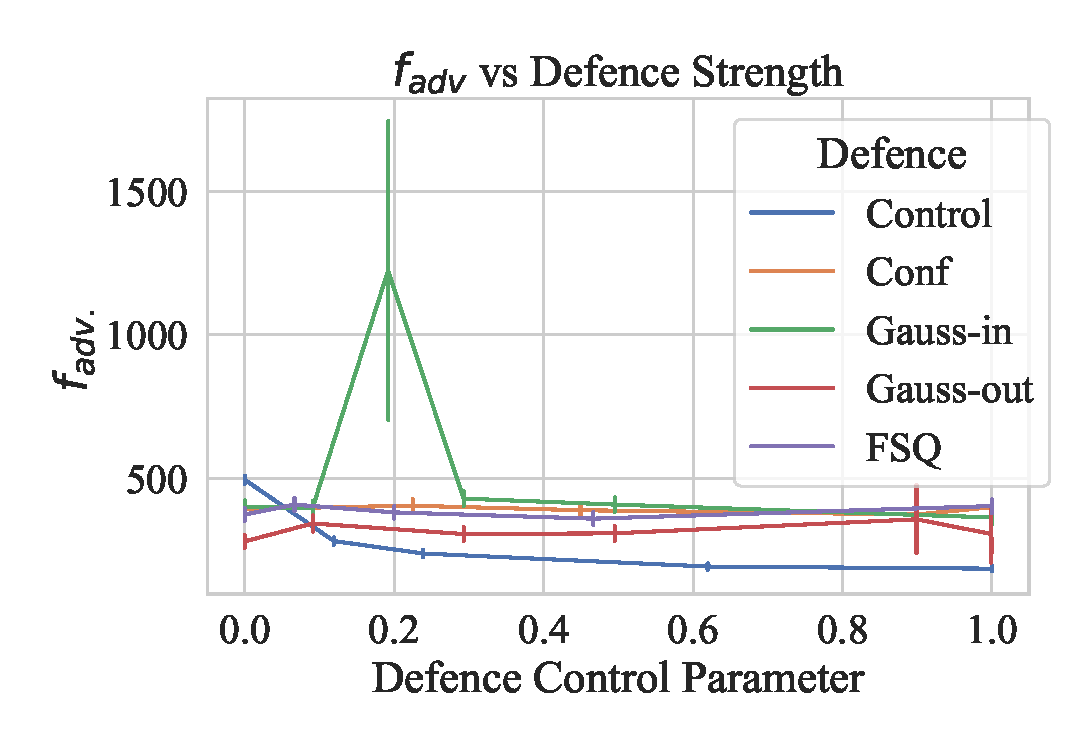
\includegraphics[width=.4\textwidth]{plots/def_param_vs_adv_failure_rate.pdf}
%     \end{subfigure}
%     \begin{subfigure}
%         \centering
%         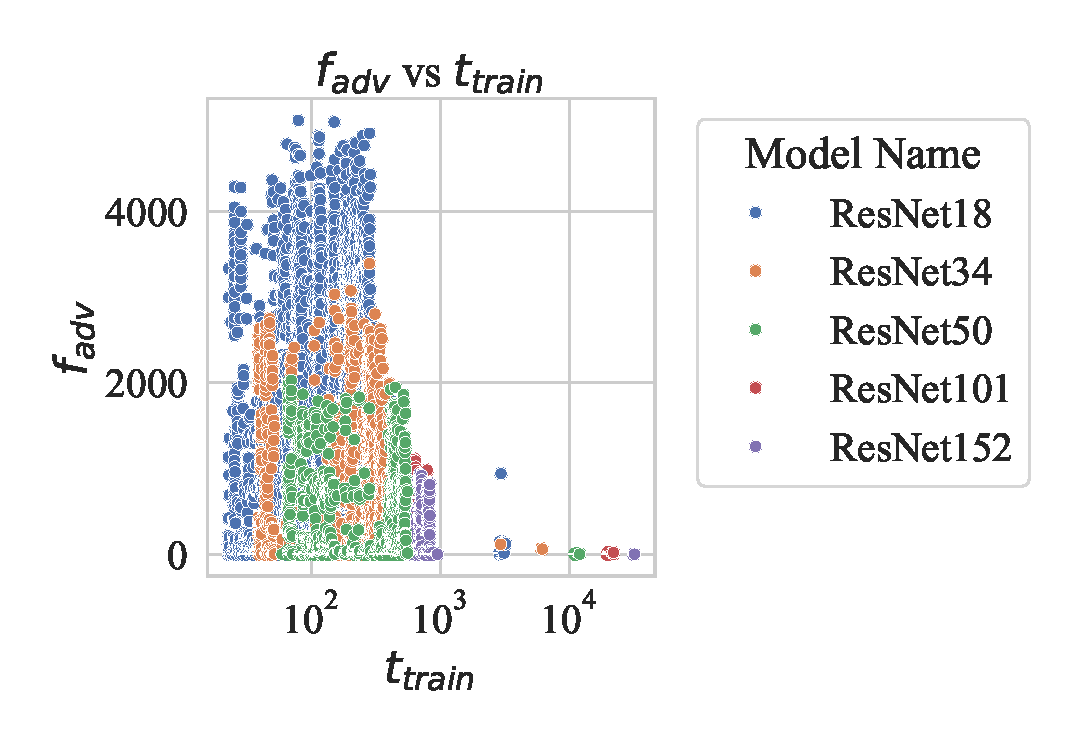
\includegraphics[width=.4\textwidth]{plots/adv_failure_rate_vs_train_time.pdf}
%     \end{subfigure}
%     \caption{The left shows the adversarial failure rate as a function of the defence strength where the control parameter represents the number of model layers. The right depicts the adversarial failure rate as a function of training time and the ResNet configuration. The bars indicate the first standard deviation of measures across all model configurations.}
%     \label{fig:failure_rate}
% \end{figure}

\begin{figure}[!h]
    \centering
    \begin{subfigure}
        \centering
        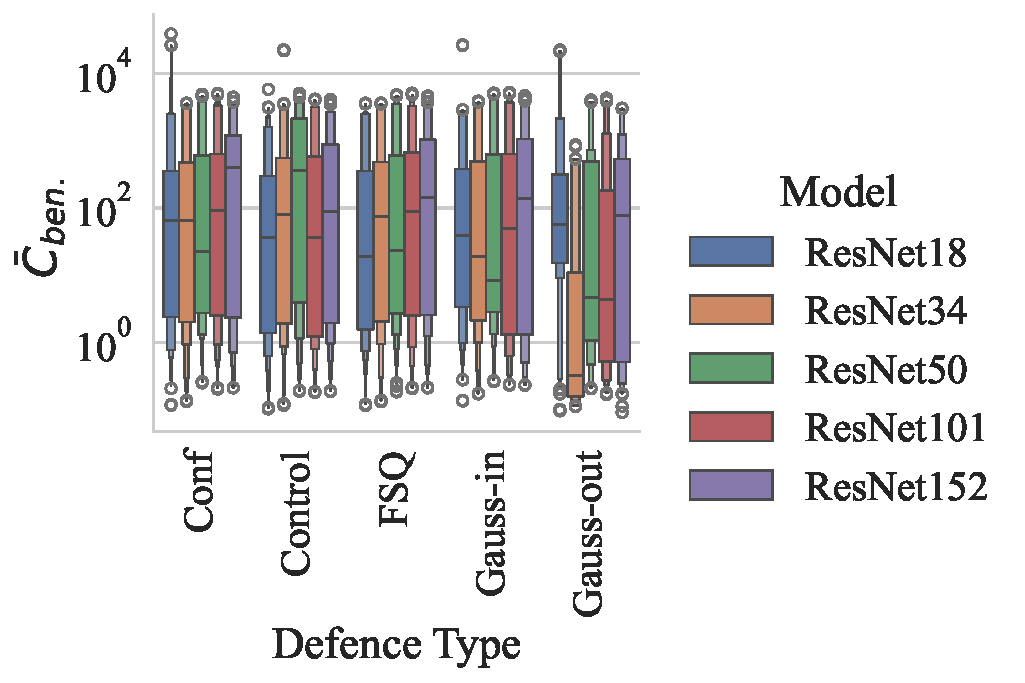
\includegraphics[width=.45\textwidth]{plots/ben_failures_per_train_time_vs_defence_type.pdf}
    \end{subfigure}
    \begin{subfigure}
        \centering
        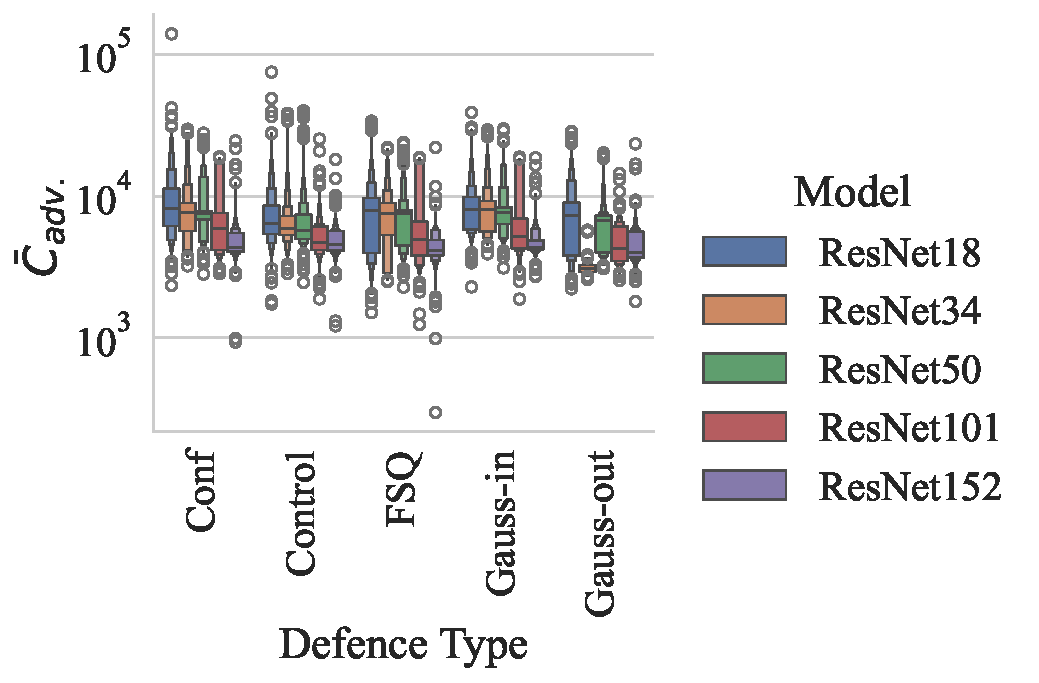
\includegraphics[width=.45\textwidth]{plots/adv_failures_per_train_time_vs_defence_type.pdf}
    \end{subfigure}
    \begin{subfigure}
        \centering
        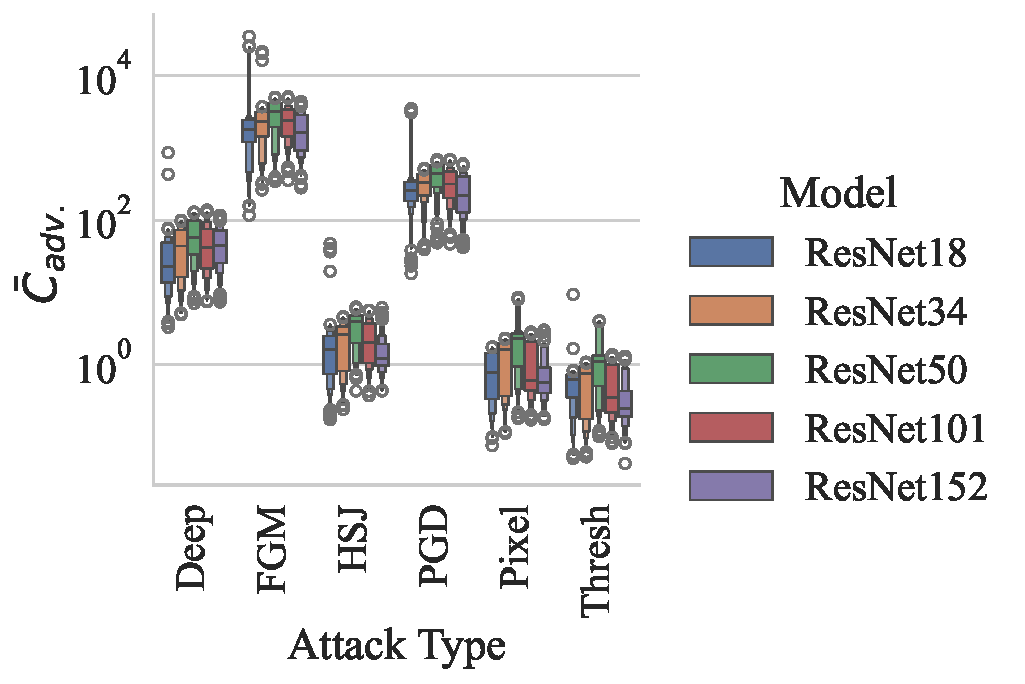
\includegraphics[width=.45\textwidth]{plots/adv_failures_per_train_time_vs_attack_type.pdf}
    \end{subfigure}
    \caption{This figure depicts the cost-normalized adversarial failure rate across a variety of defences and attacks, where training time (middle~\&~right Figs.) and inference time (left figure) is a stand-in for cost (see Section~\ref{cost}). The violin plots reflect the 95\% confidence intervals for each tuned hyperparameter combination. Outliers are indicated with a circle.}
    \label{fig:failures_per_train_time}
\end{figure}


Through tens of thousands experiments across many signal-processing techniques (\textit{e.g.}, defences), random states, learning rates, model architectures, and attack configurations, we show that model defences generally fail to outperform the undefended model in either the benign or adversarial contexts--- regardless of configuration; that the adversarial failure rate gains of larger ResNet configurations are driven by response time rather than true robustness; that these gains are dwarfed by the increase in training time; and that AFR models are a powerful tool for comparing model architectures and examining the effects of covariates. In the section below, we display and discuss the results for the CIFAR100, CIFAR10, and MNIST datasets for all attacks and defences. Fig.~\ref{fig:accuracies} depicts the benign and adversarial accuracies across the various attacks and defences. We can clearly see that no defence consistently outperforms the undefended (control) model in either the benign (top) or adversarial context (middle).



% \subsection{Attack and Defence Strength}
% In Fig.~\ref{fig:strength},  (denoted in blue). Furthermore, the relationship between the defence control parameter and the benign accuracy is not monotonic, meaning that tuning is will be expensive. We can see that the relationship between the attack parameters and failure rate is also not monotonic. However, all defences appear to perform much worse in the average adversarial case (right) than in the benign (left). Additionally we see in the right side of Fig.~\ref{fig:strength} that the attack types yield relatively consistent results, with the mean of one falling in the 95 confidence intervals of all the others. We can also see that defence choice follows the same pattern, except for Gauss-in, which rapidly decreases the accuracy as we increase the input noise.


% \subsection{Failure Rate}
% Fig.~\ref{fig:failure_rate} depicts the adversarial failure rate of all tested attacks, defences, and model configurations. 
% Clearly, increasing the depth of the model architecture does little for adversarial robustness while universally increasing the training time. 
% Furthermore, it reveals something surprising---that increasing the number of hidden layers tends to increase the failure rate---even across model architectures and all defences. 
% Certain defences can outperform the control model---at the cost of expensive tuning---evidenced by the large variance in performance (see left side of Fig.~\ref{fig:failure_rate}). The right subplot of Fig.~\ref{fig:failure_rate} shows that there is no general relationship between training time and adversarial failure rate.
% As the training time increases, however, the variance of attack times decreases, likely due to the increase in inference time (see:~\ref{fig:afr_models}) rather than inherent robustness.
% We formalize this analysis  in the next subsection.

Fig.~\ref{fig:failures_per_train_time} depicts the cost-normalized failure rate in both the benign (left) figure and adversarial cases (middle and right figures). Counter-intuitively, we see that the smallest model (ResNet18) tends to outperform both larger models (ResNet50 and ResNet152). Furthermore, we see that defence tuning is about as important as choosing the right type of defence (see: left side of Fig.~\ref{fig:failures_per_train_time}), with all defences falling within the normal ranges of each other. However, adding noise to the model output (Gauss-out) tends to underperform relative to the control for all models (see left side of Fig.~\ref{fig:failures_per_train_time}). Likewise, the intersectional relationship between model choice and optimal defence is highlighted since the efficacy of a defence depends as much on model architecture as it does on hyperparameter tuning.  Furthermore, performance across all attacks is remarkably consistent with intra-class variation being smaller than inter-class variation almost universally across defences and model configurations.



\subsection{AFR Models}

Fig.~\ref{fig:afr_models} reveals very similar estimates for the model parameters despite the models having different forms, suggesting that these parameter estimates reflect the true effect of these covariates on the failure rate. Table~\ref{tab:combined} contains the performance of each of these models on the CIFAR10 dataset. For all datasets, we can see that they are roughly comparable with regards to Concordance, but that Log-Normal model marginally outperforms the Weibull model when measured with AIC/BIC as well as the Concordance.
In all cases, the mean time until false classification is much larger than the median, indicating the long-tailed nature of these distributions.
The concordance scores for all three distributions are in agreement as well, confirming our assumption that accuracy is not independent of attack time (e.g., Concordance $> 0.5$).
We then used the Log-Normal AFR to demonstrate the partial effect of the the number of layers on the survival time as in Fig.~\ref{fig:covariates}. In that figure can clearly see that more hidden layers do increase the survival time. However, that seems to driven more by the model query time (see Fig.~\ref{fig:afr_models}) than the number of model layers.
\begin{figure*}
	% \centering
	\begin{subfigure}
		\centering
		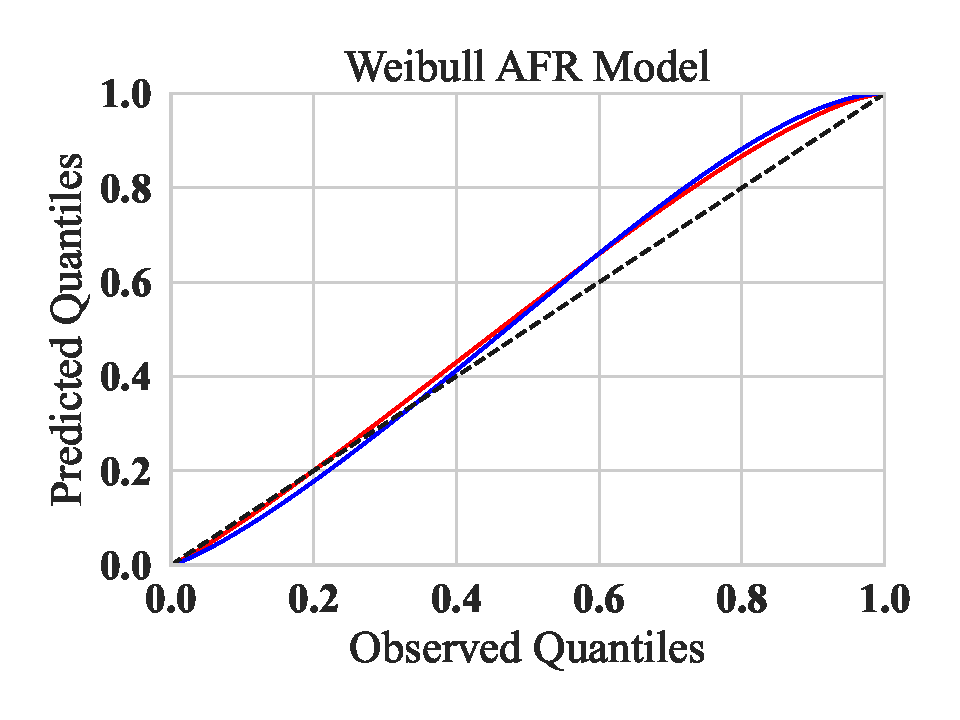
\includegraphics[width=.32\textwidth]{plots/weibull_qq.pdf}
	\end{subfigure}%
	~
	\begin{subfigure}
		\centering
		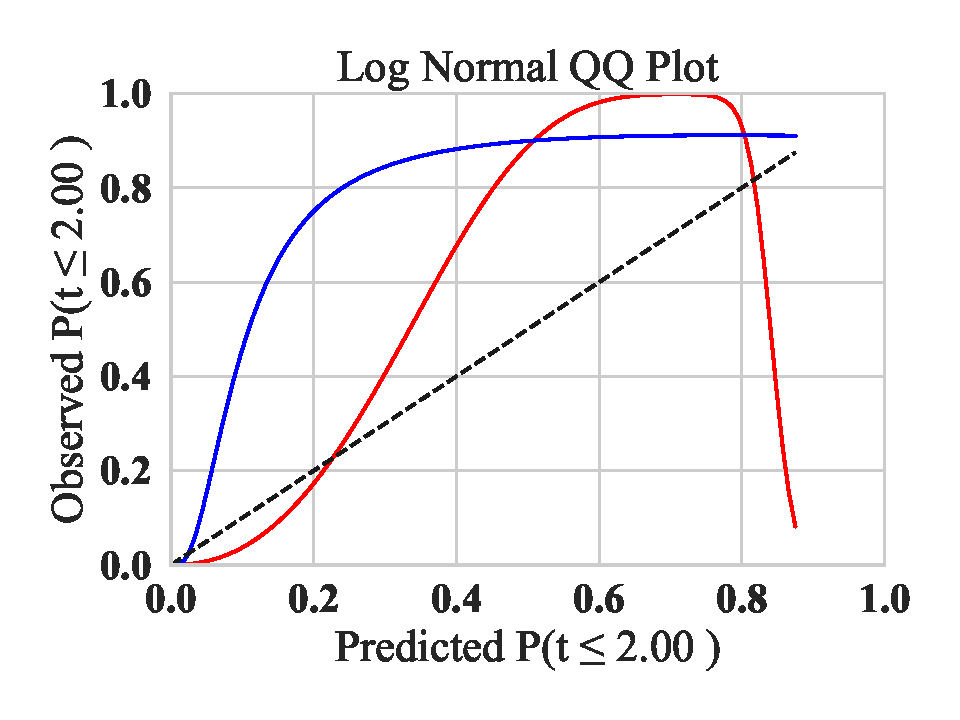
\includegraphics[width=.32\textwidth]{plots/log_normal_qq.pdf}
	\end{subfigure}
	~
	\begin{subfigure}
		\centering
		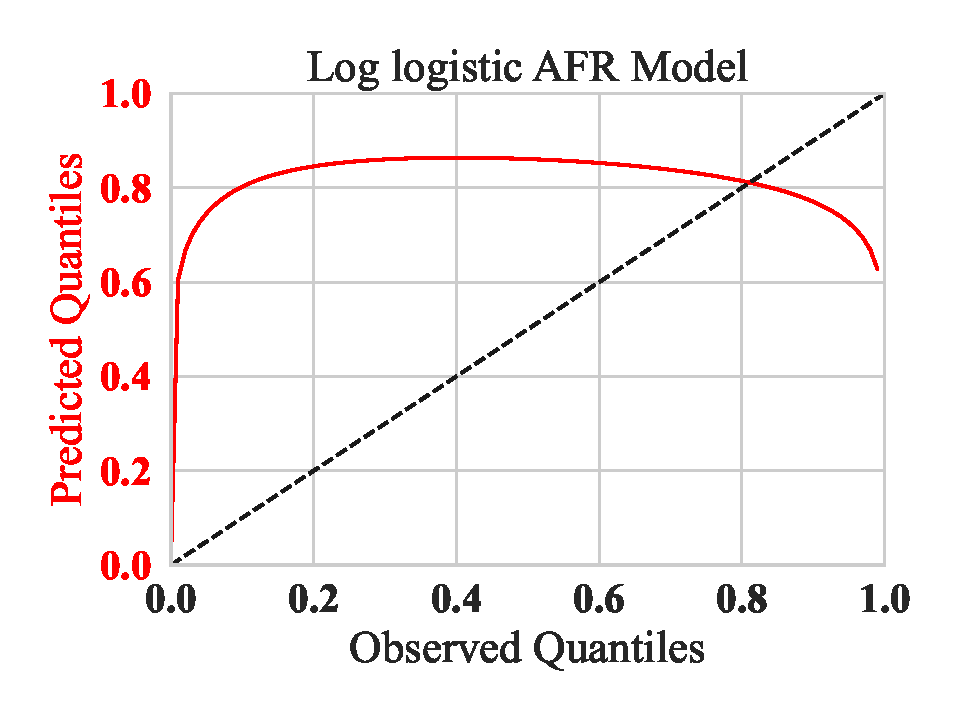
\includegraphics[width=.32\textwidth]{plots/log_logistic_qq.pdf}
	\end{subfigure}
 \begin{subfigure}
		\centering
		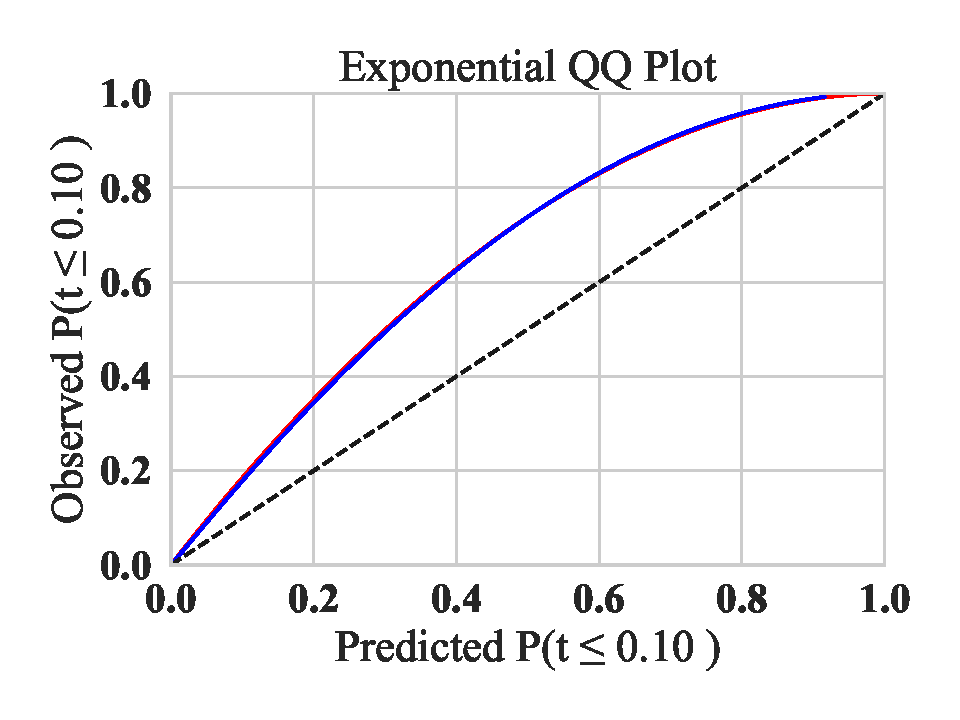
\includegraphics[width=.32\textwidth]{plots/exponential_qq.pdf}
	\end{subfigure}%
	~
	\begin{subfigure}
		\centering
		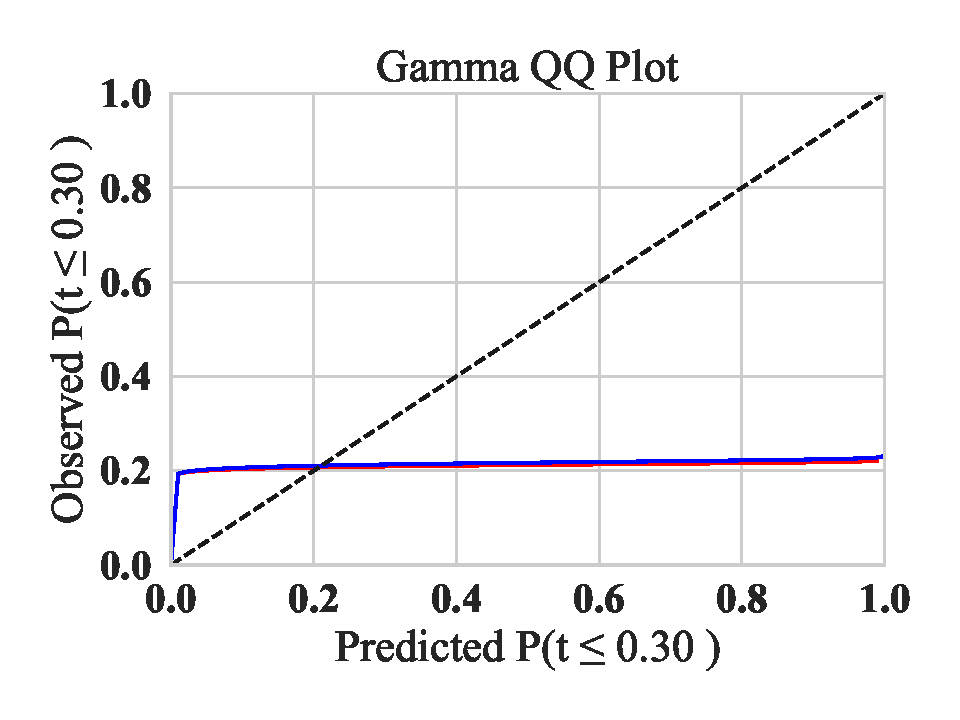
\includegraphics[width=.32\textwidth]{plots/gamma_qq.pdf}
	\end{subfigure}
	~
	\begin{subfigure}
		\centering
		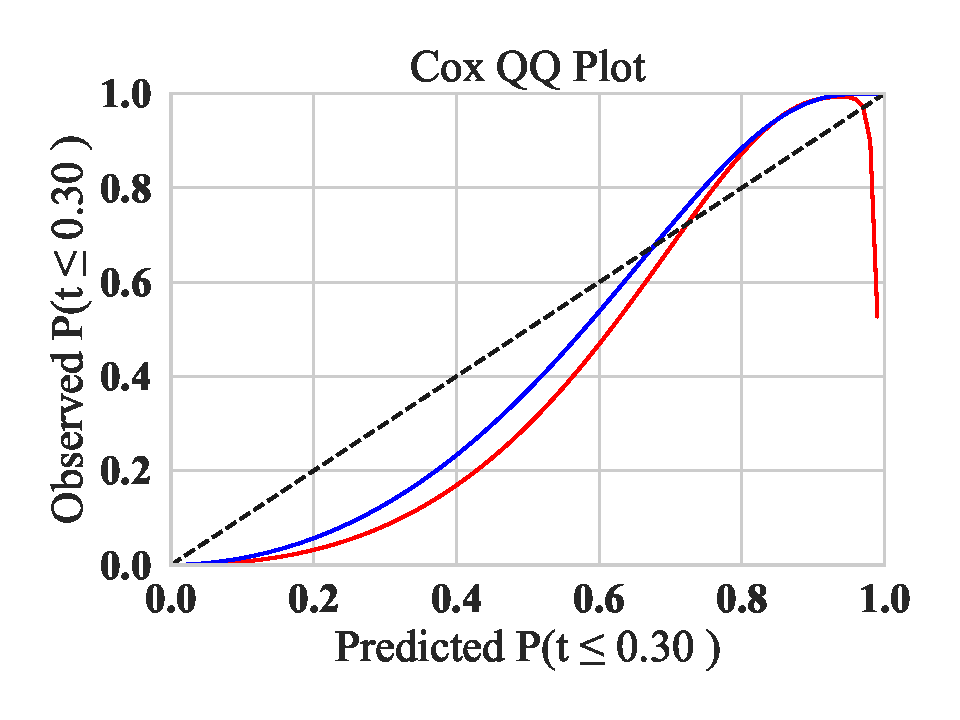
\includegraphics[width=.32\textwidth]{plots/cox_qq.pdf}
	\end{subfigure}
	\caption{These quantile-quantile plots demonstrate the efficacy of various AFR models. The first axis is the observed quantile of a sample and the second axis represents the theoretical quantile according to the chosen AFR model. The dashed black line represents a perfect fit. To verify each model, we reserved 80\% of the data to be the training set (red) and 20\% to be the test set (blue). 
 % The absence of one of the lines means that the \texttt{lifelines} fitter failed to converge for that subset.
 }
	\label{fig:afr_models}
\end{figure*}
\begin{table*}
\centering
\label{tab:afr_models}
\begin{tabular}{lllrrrrrr}
\toprule
 & AIC & BIC & Concordance & Test Concordance & ICI & Test ICI & E50 & Test E50 \\
\midrule
Cox & -- & -- & 0.92 & 0.92 & 0.06 & 0.27 & 0.04 & 0.08 \\
Gamma & -- & -- & 0.51 & 0.52 & 0.26 & 0.43 & 0.17 & 0.32 \\
Weibull & 9.05e+04 & 9.05e+04 & 0.92 & 0.92 & 0.02 & 0.2 & 0 & 0.01 \\
Exponential & 7.93e+04 & 7.93e+04 & 0.86 & 0.86 & 0.04 & 0.2 & 0 & 0.02 \\
Log Logistic & 9.79e+04 & 9.79e+04 & 0.92 & 0.92 & 0.07 & 0.08 & 0.01 & 0.01 \\
Log Normal & 1.14e+05 & 1.14e+05 & 0.91 & 0.91 & 0.15 & 0.26 & 0.08 & 0.19 \\
\bottomrule
\end{tabular}
\end{table*}

\begin{figure}
    \centering
	\begin{subfigure}
	\centering
    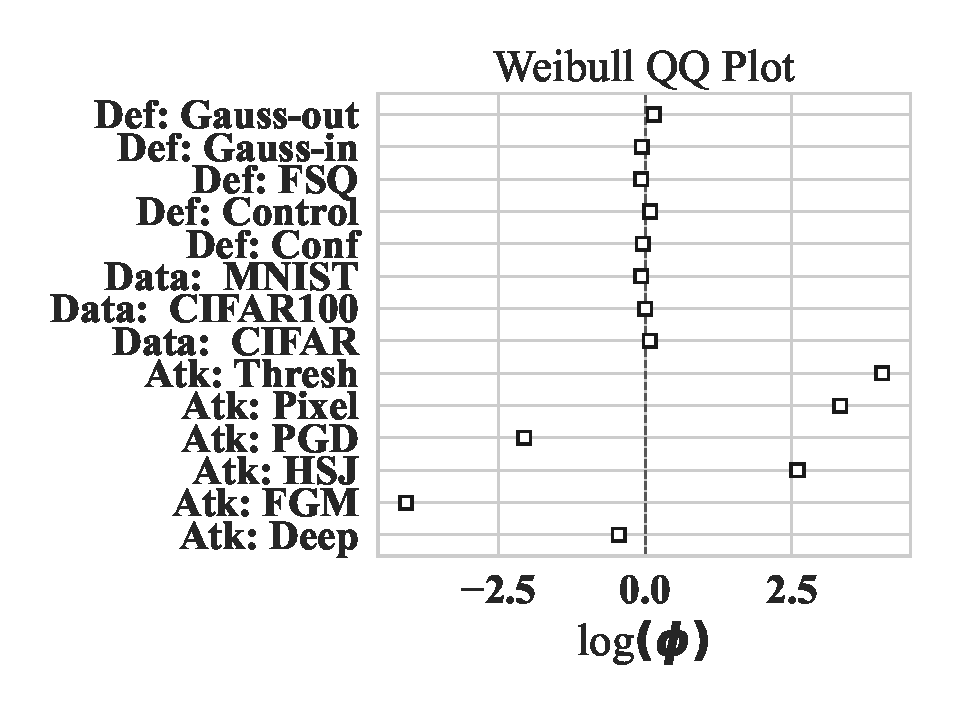
\includegraphics[width=.38\textwidth]{plots/weibull_aft_dummies.pdf}
    \label{fig:covariates}
    \end{subfigure}
    \begin{subfigure}
	\centering
    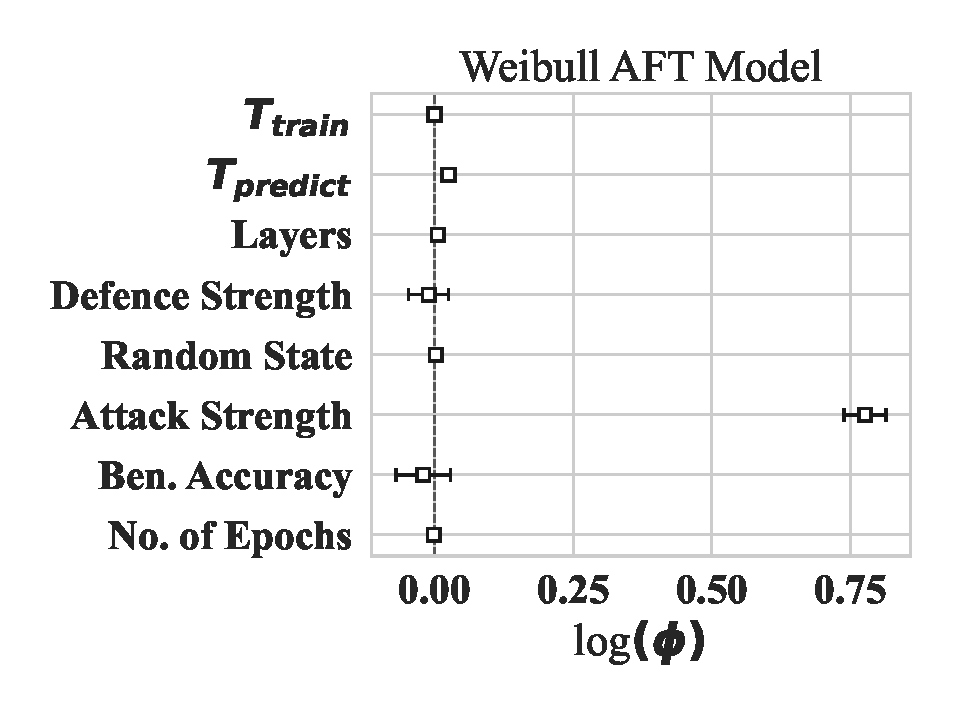
\includegraphics[width=.38\textwidth]{plots/weibull_aft.pdf}
    \label{fig:dummies}
    \end{subfigure}
    \caption{The coefficients represent the log scale effect of the dummy variables for dataset, attack, and defence on the survival time, with a positive value indicating an increase in the survival time.}
\end{figure}




\section{Considerations}
The proposed survival and cost analysis  has some limitations that we have taken all efforts to minimise and/or mitigate. 
In order to minimise timing jitter, we measured the process time for a batch of samples and then assumed that the time per sample was the measured processor time divided by the number of samples. 
In order to examine a variety of different optimisation criteria for adversarial perturbations, we included several different attacks (see Section~\ref{attacks})---though the choice of attack is highly contextual.
We must also note that none of these attacks are run-time optimal and are, at best, an underestimate of the true adversarial failure rate~\cite{meyers}. 
Likewise, testing all known defences would be computationally infeasible. 
As such, we focused only on the pre- and post-processing technique. 
% Techniques like adversarial retraining~\cite{croce_reliable_2020}, model transformation~\cite{papernot_distillation_2016}, and model regularisation~\cite{jakubovitz2018improving} were excluded due to their comparatively larger run-times. The equation Section~\ref{cost_normalization} reveals why techniques that significantly increase the training time might ultimately work against the model builder.
% Even if one assumes there is a defence that has 99\% efficacy, rather than the, at best, 40\% efficacy indicated by the adversarial accuracy in Figure~\ref{fig:accuracies}, it would only reduce $\bar{C}_{\mathrm{adv}}$ by roughly two orders of magnitude.
While every configuration of ResNet met the bare minimum requirement outlined in Equation~\ref{eq:cost}, real training processes require many thousands of samples and attacks are consistently successful with only one hundred samples. 
Together, these considerations raise serious concerns about the efficacy of any of these models and defences in the presence of these simple adversaries, meaning attacks will likely be many orders of magnitude cheaper than defences for tested configurations of this model.
Furthermore, state of-the art leaderboards\footnote{\href{https://github.com/MadryLab/mnist\_challenge}{Madry's MNIST Challenge}}\footnote{\href{https://ml.cs.tsinghua.edu.cn/adv\-bench/}{Croce's Robust Bench}}
show that a 99\% generalised adversarial accuracy is, at best, optimistic. 
% Nevertheless, the goal of this work was not to produce a comprehensive evaluation of all known defences, but to develop a cost-aware framework for evaluating their efficacy against a set of adversaries.

\section{Conclusion}
Convolutional neural networks have shown to be widely applicable to a large number of fields when large amounts of labelled data are available.
By examining the role of the attacks, defences, and model depth in the context of adversarial failure rate, this paper presents a reliable and effective modelling framework that applies AFT models to deep neural networks.
The metrics outlined Table~\ref{tab:aft_summary} and explained in Section~\ref{metrics} show that this method is both effective and data-agnostic.  
We use this model to demonstrate the efficacy of various attack- and defence-tuning techniques, to  explore the relationships between accuracy and adversarial robustness (Figure~\ref{fig:dummies}), and show that various model defences are ineffective on average and marginally better than the control at best.
By measuring the cost-normalised failure rate or TRASH score (see Section~\ref{cost_normalization} and Figure~\ref{fig:trash}), it is clear that all tested configurations of ResNet fail to meet the TRASH criterion.
The methods can easily extend to any other arbitrary collection of model pre-processing, training, tuning, attack and/or deployment parameters. 
In short, AFTs provide a rigorous way to compare not only the relative robustness of a model, but of its cost effectiveness in response to an attacker.
The measurements rigorously demonstrate  that the depth of a ResNet architecture does little to guarantee robustness while the community trends towards larger models~\cite{desislavov2021compute}. 

While the train-test split methodology relies on an ever-larger number of samples to increase precision, the survival time method is able to precisely and accurately compare models using only a small number of samples~\cite{schmoor2000sample,lachin1981introduction} relative to the many billions of samples required of the train/test split methodology and safety-critical standards~\cite{iso26262,IEC61508,IEC62034,meyers}.
In short, by generating worst-case examples (\textit{e.g.}, adversarial ones), one can test and compare arbitrarily complex models \textit{before} they leave the lab, drive a car, predict the presence of cancer, or pilot a drone.

\printbibliography
\end{document}

